\documentclass[border=10pt]{standalone}

\usepackage{tikz}
\usepackage{tikzsymbols}
\usetikzlibrary{calc,patterns,shapes.geometric}

\def\centerarc[#1](#2)(#3:#4:#5){\draw[#1] ($(#2)+({#5*cos(#3)},{#5*sin(#3)})$) arc (#3:#4:#5);}

\begin{document}
	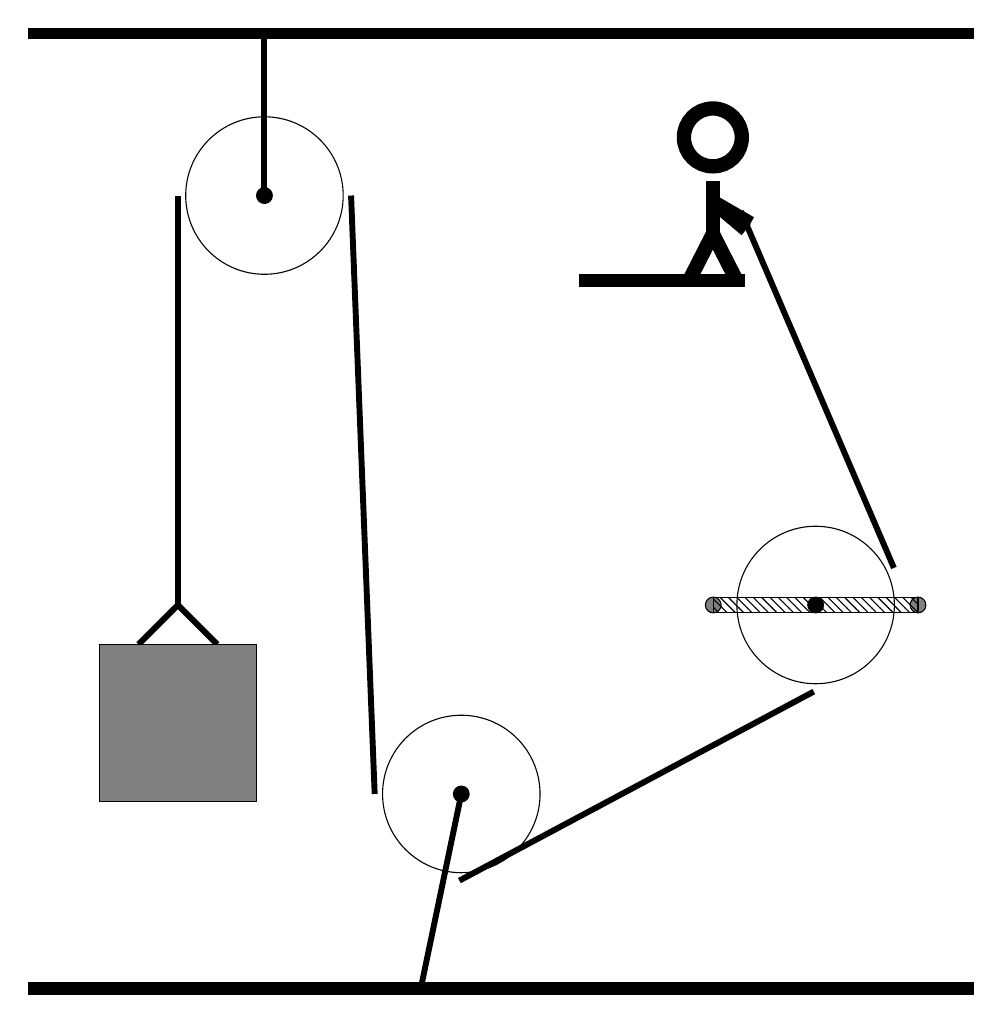
\begin{tikzpicture}
		%%%%% START %%%%%
		\draw[fill=black] (-2, 12) rectangle (10, 12.125);
		
		\draw (1, 10) circle (1);
		\draw[fill=black] (1, 10) circle (0.1);
		\draw[line width=0.75mm] (1, 12) -- (1, 10);
		
		\draw (3.5, 2.4) circle (1);
		\draw[fill=black] (3.5, 2.4) circle (0.1);
		\draw[line width=0.75mm] (3.5, 2.4) -- (3.0, 0);
		
		\draw[fill=white](8, 4.8) circle (1);
		\draw[fill=black] (8, 4.8) circle (0.1);
		\draw[fill=black!50] (9.3, 4.8) circle (0.1);
		\draw[fill=black!50] (6.7, 4.8) circle (0.1);
		\draw[pattern=north west lines, pattern color=black] (6.7, 4.9) rectangle (9.3, 4.7);
		
		\draw[line width=0.75mm](-0.6, 4.3) --  (-0.1, 4.8) -- (0.4, 4.3);
		\draw[fill=black!50] (-1.1, 4.3) rectangle (0.9, 2.3);
		
		\draw[line width=0.75mm](-0.1, 10) -- (-0.1, 4.8);
		\centerarc[line width=0.75mm](1, 10)(180:0:1.1)
		\draw[line width=0.75mm](2.1, 10) -- (2.4, 2.4);
		\centerarc[line width=0.75mm](3.5, 2.4)(180:300:1.1);
		\draw[line width=0.75mm](3.476, 1.3) -- (7.976, 3.7);
		\centerarc[line width=0.75mm](8, 4.8)(300:390:1.1);
		\draw[line width=0.75mm](8.994, 5.271) -- (7.05, 9.8);
		
		\node at (6.75, 10) {\Strichmaxerl[10][-220][-30]};
		\draw[fill=black] (5, 9) rectangle (7.1, 8.85);
		
		\draw[fill=black] (-2, 0) rectangle (10, -0.15);
		%%%%% END %%%%%
	\end{tikzpicture}
\end{document}